\section{CCTF Secure Server}
\label{sec:cctf-secure}

\subsection{Scenario}
\label{sec:cctf-secure:scenario}

The network structure was identical to the Resilient Server CCTF (\autoref{sec:cctf-resilient:scenario}). The only difference was that the router was performing Network Address Translation (NAT), and we noticed that only during the competition. 
For the blue team, this implied that every incoming packet had the source IP of the router (\texttt{10.1.1.2}).

The \textit{server} had a LAMP stack configured with Apache, MySQL, and PHP.  
There were exposed APIs for a bank system accepting HTTP GET requests to create new users, fetch the balance, withdraw or deposit money.
The \textit{gateway} was left free to be customized by the blue team. 

During the CCTF, some bank customers actively made requests and interacted with the bank APIs. Only the blue team knew the customers' names, not the red one. The blue team's goal was to operate the bank system correctly and keep the database consistent without being fined or robbed by the red team.

On the attack side, the three clients at the red team's disposal had only one limitation about traffic floods of one request per second. However, short bursts were allowed as long as the red team respected the limit over time (e.g., ten requests in a second then silent for nine seconds). 

The red team had infinite money and could freely create new users and interact with them. Their ultimate goal was to rob the bank with compromising requests, asking for ransoms, or forcing the bank to pay fines \cite{secure-server}.

\subsection{Environment setup}
\label{sec:cctf-secure:env-setup}

Our previous setup, used in the Resilient CCTF and described in  \autoref{sec:cctf-resilient:env-setup}, was again employed for this CCTF.

\subsection{Attack preparation}
\label{sec:cctf-secure:att-prep}

\subsubsection{Goals}
\label{sec:cctf-secure:att-prep:goals}

The red team's goal was to steal as much money as possible from the bank. Several approaches were possible to achieve this goal:

\begin{itemize}
    \item Deleting or corrupting users' accounts via malicious requests to the APIs.
    \item Compromise the database and lead it into unexpected behavior (e.g., reducing a user balance below zero, creating money out of nowhere).
    \item Bring the server down to a halt.
\end{itemize}

Except for flooding techniques, it was possible to use any means to achieve such goals. For example, brute forcing any blue team member's password was allowed.

\subsubsection{Tools used}
\label{sec:cctf-secure:att-prep:tools-used}

Since flooding was not allowed in this CCTF, we actively searched for exploits in the unpatched PHP and MySQL code provided to the blue team.

To help in our analysis, we used two main tools:

\begin{itemize}
    \item \texttt{Nmap}~\cite{nmap}: a utility for network discovery and security auditing. It is used by white and black hat hackers alike in settings that range from reconnaissance to vulnerability discovery;
    \item \texttt{SQLMap}~\cite{sqlmap}: a penetration testing tool that automates the process of detecting and exploiting SQL injection flaws. When provided with an URL that supports query strings, \texttt{SQLMap} sequentially checks relevant injections and provides results to the user.
\end{itemize}

Slow DoS attacks were permitted, enabling us to use \texttt{Sockstress}~\cite{github:sockstress} and \texttt{SlowLoris}~\cite{github:slowloris}.

To automate the requests to the web server, we developed \texttt{Attila}: a bash function with log functionalities that made possible to send requests to the server in a one-liner. This tool allowed us to create powerful scripts with minimal boilerplate code. An example of usage is the following which sends a request to the server and logs the response time:

\begin{verbatim}
    attila "random_user" "user_s_password" "withdraw" "100"
\end{verbatim} 

A few hours before the CCTF, we tried a social engineering attack (described in \autoref{sec:cctf-secure:att-prep:strat-out}) using \texttt{Emkei's Fake Mailer}~\cite{emkei}, a website that allows anyone to send forged emails with customized fields (e.g., sender, attachments, signature).

\subsubsection{Strategy overview}
\label{sec:cctf-secure:att-prep:strat-out}

Unlike the Resilient Server CCTF, we had almost no idea where to start, so we decided on a more generic and planned strategy, outlining it step-by-step. Then we divided the work between the team members, looking for different vulnerabilities.

\begin{enumerate}[1.]
    \item At the beginning of the CCTF, use tools such as \texttt{Nmap} and \texttt{SQLMap} to test the capabilities of the adversarial system, looking for open ports and vulnerabilities.
    \item After narrowing down the attack surface, choose the priority of the following attacks: \begin{enumerate}[a.]
        \item \textbf{Dictionary attacks}: brute force any of the opposing team's passwords, such as their deterlab SSH passwords or the legitimate bank users' passwords.
        \item \textbf{Database flood}: flood the opposing system with a large number of user registration requests to enlarge the database tables enough to slow down the queries and the system.
        \item \textbf{Discovery}: verify the presence of additional pages on the system, possibly forgotten, and try to compromise them.
        \item \textbf{Corner case checking}: send crafted requests to the web server to crash it or trigger odd behavior. Test for SQL injection and XSS strings, then use \texttt{Attila} scripts to check edge cases such as empty requests, empty username requests, strange Unicode characters, and more.
    \end{enumerate}
    \item Use the aforementioned \texttt{Emkei's Fake Mailer} to send a phishing email, pretending to be the Teaching Assistant. The email would contain instructions to set a specific root password for the database and create ``default’’ bank users.\footnote{We had the phishing email idea only a few hours before the CCTF. We report it here for completeness.} The email text is reported in Attachment~\ref{sec:attachments:phishing}.
\end{enumerate}

\subsection{Defense preparation}
\label{sec:cctf-secure:def-prep}


\subsubsection{Goals}
\label{sec:cctf-secure:def-prep:goals}

The blue team's goals were to ensure 100\% server availability over time and to preserve the database integrity. 
The server had to serve all the requests, and any timed-out request was marked as disputed and verified later. 
The database had to be as resilient as possible, with the underlying PHP code blocking any incorrect database query.

Moreover, the bank had to comply with different policies such as \textit{KYC} requirements (unique customer identification), transactions logging, and data privacy. Violating any of these policies would result in a fine, ultimately decreasing the team's total score.

\subsubsection{Strategy overview}
\label{sec:cctf-secure:def-prep:strat-out}

We changed the server configuration to an LNMP stack with Nginx, MySQL, and PHP, thus removing the Apache web server.
The provided PHP code was poorly written, with no input validation, plaintext passwords, and any other problem we could think of.
The first part of the work was to fix the source code while preserving the APIs functionalities and the log structure.

Then, due to the packets rate restriction, our strategy focused on hardening the LNMP stack on the server rather than handling floods on the gateway like in the Resilient Server CCTF.

\paragraph{Gateway}
\label{sec:cctf-secure:def-prep:gateway}

We set up the gateway as the first line of defense, configuring the firewall with a default \texttt{DROP} policy and allowing everything on the DETERLab interface and only TCP traffic coming from the router to the server on port 80. The \texttt{iptables} configuration was similar to the one mentioned in \autoref{sec:cctf-resilient:def-prep:gateway} but without the \texttt{raw} and the \texttt{mangle} tables rules.
We also limited at a maximum of ten parallel connections per IP.

\paragraph{Server}
\label{sec:cctf-secure:def-prep:server}

We decided to use Nginx to have a lighter web server that could handle loads and multiple connections better than Apache without requiring additional modifications. Also, using Nginx instead of Apache should have theoretically reduced the complexity of hardening our configuration, but in reality, we had a tough afternoon making the LNMP stack work flawlessly.

We hardened the database following the security guidelines provided by \texttt{MySQL}~\cite{Mysql:securityguidelines}.

We refactored the PHP code entirely, adding a multi-layer input validation and filtering. We filtered all the input parameters using \texttt{htmlentities}, then we used the \texttt{filter\_var} function to check for odd strings or integers. Finally, we changed all the queries to prepared statements.

On top of this filtering, we added checks for negative amounts, integer overflow, user existence (to avoid duplicate users), and password hashing using the \texttt{ARGON2I} algorithm \cite{argon2i}.

\paragraph{Database}
\label{sec:cctf-secure:def-prep:database}

We kept MySQL, disabling local file access and introducing an incremental delay after each failed login attempt to the database. Remote access was already disabled.

We rebuilt the database as shown in \autoref{fig:cctf-ss-db}. A user was identified through a unique username and could have zero or more transfers. Randomly-generated 32-bit unique identifiers distinguished transfers, and each transfer could be associated with one and only one user.

\begin{figure}[h]
    \centering
    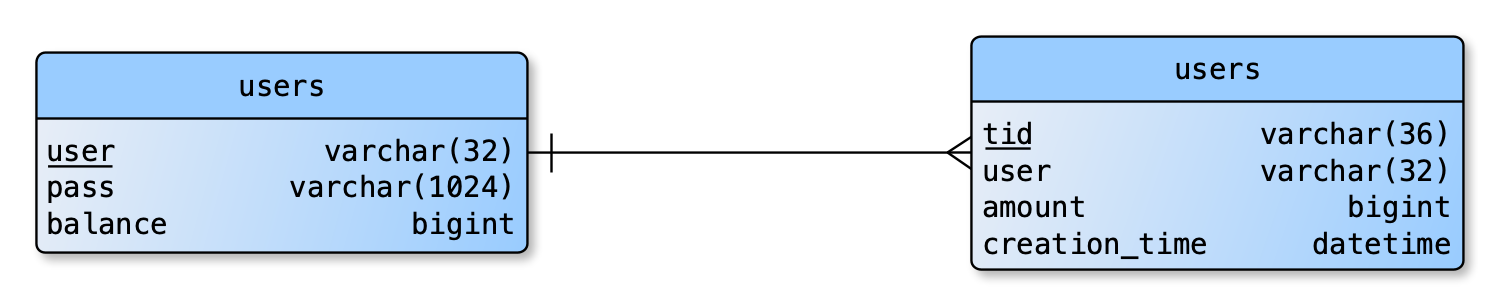
\includegraphics[width=0.6\textwidth]{drawable/db_diagram.png}
    \captionsetup{justification=centering}
    \caption{Database ER diagram.}
    \label{fig:cctf-ss-db}
\end{figure}

We set up three different users: a \textit{root user} with complete access to the database, an \textit{editor user} with \texttt{INSERT}, \texttt{SELECT} and \texttt{UPDATE} privileges on our two tables, and a \textit{monitor user} to check the database consistency and perform backups.

\paragraph{Monitoring}
\label{sec:cctf-secure:def-prep:monitoring}

Again, as in the Resilient Server CCTF, we developed monitoring tools in Python. Since DoS attacks were not allowed, we focused on the integrity of the database.

\begin{itemize}
    \item \texttt{database\_checker.py}: a script that checked the consistency of the database every 60 seconds. It connected to the database with the \textit{monitor user} and performed four checks:
    \begin{itemize}
        \item \textit{Negative amount}: the sum of the transfers values of any user could have not been negative. If a user had a negative balance, it displayed the correspondent username on the screen.
        \item \textit{Number of transfers and users}: the number of users and transfers should have never decreased since we did not allow the delete command.
        \item \textit{Matching balance}: each user's balance should have matched the sum of their transfers. In case of incongruences, the corresponding username was displayed on the screen.
    \end{itemize}
    The script also monitored the MySQL log file, displaying an alert in case of any failed attempt to connect to the database. Moreover, we added a backup function to save the entire database and the \texttt{request.log} file if the former was intact. During the CCTF, we kept the three most recent backups.
    \\
    This tool allowed us to control the database consistency and offered a quick way to restore everything in case of a successful attack.
    \item \texttt{traffic\_logger.py}: we reused the \texttt{traffic\_logger} developed for the Resilient Server CCTF without modifications. It helped us understand that the router was doing NAT.
\end{itemize}

\subsection{Execution}
\label{sec:cctf-secure:exec}

\subsubsection{Attack}
\label{sec:cctf-secure:exec:att}
 
In this CCTF, the attack part was a failure. Our strategy mostly followed the plan, but unfortunately, we could not compromise anything on the blue team side, and thus we did not steal any money.

As a last-minute idea, we tried our luck with a phishing email (Attachment \ref{sec:attachments:phishing}). To make it appear as realistic as possible, we added the Teaching Assistant's signature, removed any attachments triggering Gmail's spam filters, and sent one copy to the other two team leaders. Our plan failed because Team 1 asked the Teaching Assistant for clarification and thus spoiled the phishing attempt to Team 2, whose leader did not even check his incoming email.

In the initial part of the CCTF, we deployed \texttt{Nmap} and \texttt{SQLMap} scans as planned. We additionally used \texttt{Nmap}'s vulnerability scanners, hoping to find some exploitable vulnerabilities. Unfortunately, we had no luck. Not only were all SQL injection and XSS attempts blocked, but the scan yielded no vulnerability exploitable in a reasonable amount of time.

We split the job and started working on the side channels with no other options left. Using \texttt{Attila}, we flooded the database with a list of a million users to inject them into the opponent's database. However, the slow one-request-per-second rate meant that only a small fraction of the users made their way into the system. At a certain point, we spotted an already registered user, thus triggering the second step of our plan.

We equipped our \texttt{BruteForcer} script with a list of common passwords and ran it against the web server. In the end, maybe also because of the limited rate, we could not guess the user's password.

Meanwhile, another member of the team tried different side-channel tactics. After failing to discover secondary pages on the web server, he checked for corner cases such as integer parsing, empty usernames or passwords, and other odd combinations.
He tried using Unicode sequences and international characters as the last stand. Unfortunately, nothing of the above worked.

After the end of the competition, the professor revealed that our blue team missed a severe vulnerability and that our red team almost managed to exploit it unknowingly during the database flooding. 
The size of the log file had a quadratic growth. So, by increasing the dimension of the tables in the database, the size of the log file would increase, eventually causing the server to halt during the logging procedure. Unfortunately, the strict request rate limit and the fact that we started late to flood the database resulted in us not exploiting this vulnerability.

\subsubsection{Defense}
\label{sec:cctf-secure:exec:def}

Our defenses defied the opposing red team attacks. The monitoring tools reported no compromise, and the Teaching Assistant later confirmed this. Unfortunately, we misconfigured something initially, ending up missing some requests. Some were flagged as disputed and later resolved, but others went lost.

First, we forgot to allow DNS traffic on the gateway when configuring the firewall. Without DNS traffic, the gateway was cut out entirely from the DETERLab network for a few minutes before we could realize what was happening. All the incoming requests in that timeframe went inevitably lost.

Second, the concurrent connections limit did more harm than good. We set up the firewall to allow a maximum of ten parallel connections from the same IP. However, we did not notice that the router was performing NAT, so when the red team started attacking us with \texttt{Sockstress}, thus opening several parallel connections, our firewall blocked almost all the legitimate ones due to the abovementioned rule.

We took a while to realize what was happening because everything was running fine from our standpoint. The only weird thing is that we were receiving only traffic from the router, but we thought the Teaching Assistant was sending it, so we were not alarmed.
\clearpage
\newpage